\documentclass[11pt,a4paper]{article}
\usepackage[utf8]{inputenc}
\usepackage[german]{babel}
\usepackage{amsmath}
\usepackage{amsfonts}
\usepackage{subfig}
\usepackage{amssymb}
\usepackage{siunitx,physics}
\usepackage{mathtools}
\usepackage{graphicx}
%\usepackage{Here}
\usepackage[version=4]{mhchem}
\usepackage{url}
\usepackage{setspace}
\usepackage[left=2.5cm,right=2.5cm,top=2.5cm,bottom=2cm]{geometry}
[biblography=totocnumbered]
\usepackage{fancyhdr}
\usepackage{scrextend}
\usepackage{hyperref}
\pagenumbering{gobble}

\makeatletter
\newcommand\bigcdot{\mathpalette\bigcdot@{.5}}
\newcommand\bigcdot@[2]{\mathbin{\vcenter{\hbox{\scalebox{#2}{$\m@th#1\bullet$}}}}}
\makeatother

\makeatletter
%\renewcommand*\bib@heading{%
%  \subsection*{}%
%  \@mkboth{\refname}{\refname}}
%\makeatother
\numberwithin{equation}{section}
\numberwithin{figure}{section}

\renewcommand{\labelitemii}{\labelitemfont$\vartriangleright$}
\begin{document}\\
\begin{addmargin}[25pt]{0pt}
Silikatmaterialien bestehen aus \ce{(SiO4)^4-}-Tetraedern. Die Klassifizierung erfolgt dann nach der Anordnung dieser Tetraeder. Siliziumdioxid hat die Eigenschaft, dass benachbarte Tetraeder 2 O-Atome an ihren Ecken sich teilen, dadurch ist das gesamte 3-dimensionale Netzwerk elektrisch neutral. Siliziumdioxid hat eine sehr starke Bindung wodurch es eine hohe Schmelztemperatur besitzt. Silikatische Gläser sind in Abbildung \ref{fig:Silikatgläser} dargestellt. Auf der linken Seite sieht man ein reines Silikatglas und rechts Fensterglas, das sind Silikatgläser denen andere Materialien wie \ce{CaO} oder \ce{Na2O} zugegeben wurden.
\begin{figure}[h]
    \centering
    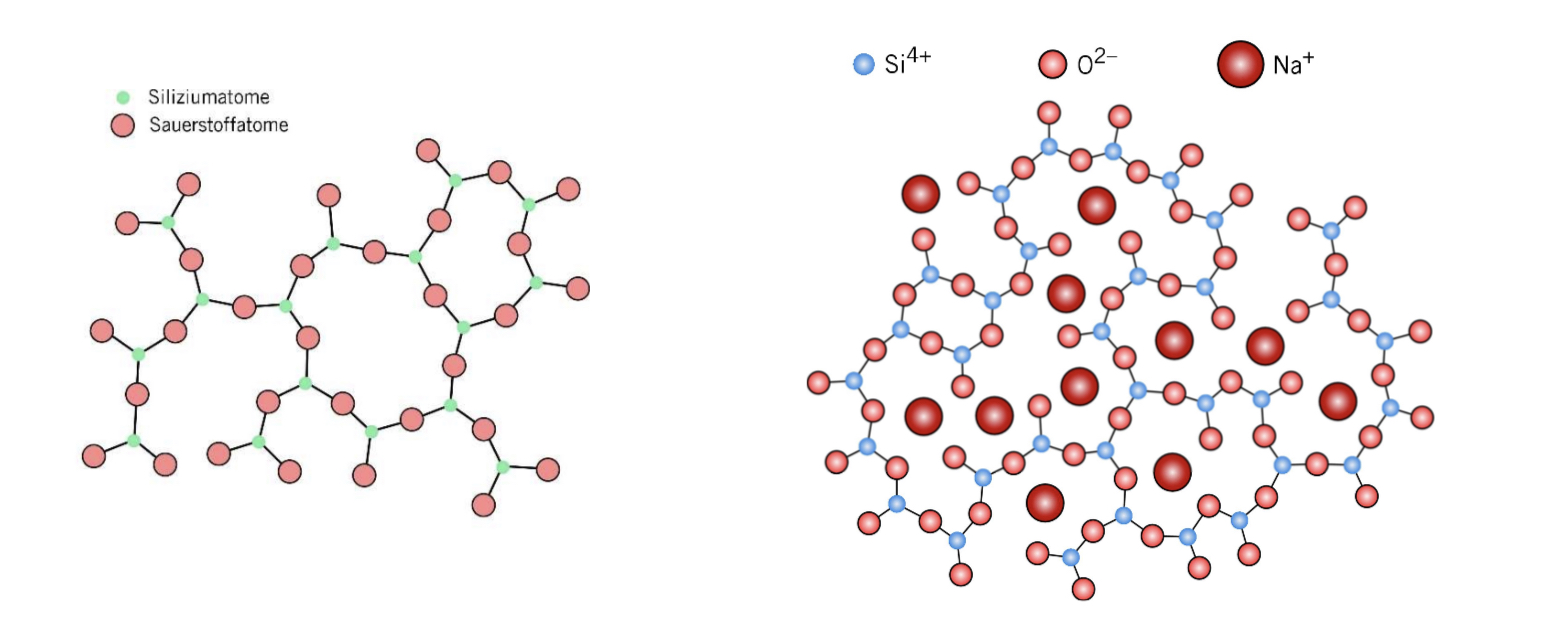
\includegraphics[width = 0.8\textwidth]{images/Materialwissenschaften/Silikatische_glaser.jpeg}
    \caption{Silikatgläser, rein auf der linken Seite und mit Zusatz rechts}
    \label{fig:Silikatgläser}
\end{figure}
Schichtsilikate sind die letzte Form der Silikatmaterialien, bei ihnen liegt eine zweidimensionale Schichtstruktur vor, bei der drei oder vier O-Atome an Tetraederecken gemeinsam genutzt werden, es entstehen \ce{(Si2O5)^2-} Verbindungen. Ein bekanntes Beispiel für ein Schichtsilikat ist der Ton.\\
\end{addmargin}

\end{document}